\chapter{Introduction}
\indent
	This task is to implement Conditional Variational AutoEncoder (CVAE) with Recurrent Neural Network (RNN), 
	concretely, Long Short-Term Memory (LSTM), to solve video prediction problem (See Figure \ref{architecture}). \\
	Bair robot pushing small dataset is used to train and evaluate the model. 
	The dataset contains roughly 44,000 sequences of robot pushing motions, and each sequence includes 30 frames. \\
	Section \ref{sec-derivation-cvae} is derivation of CVAE objective function.

	\begin{figure}[H]
		\centering
		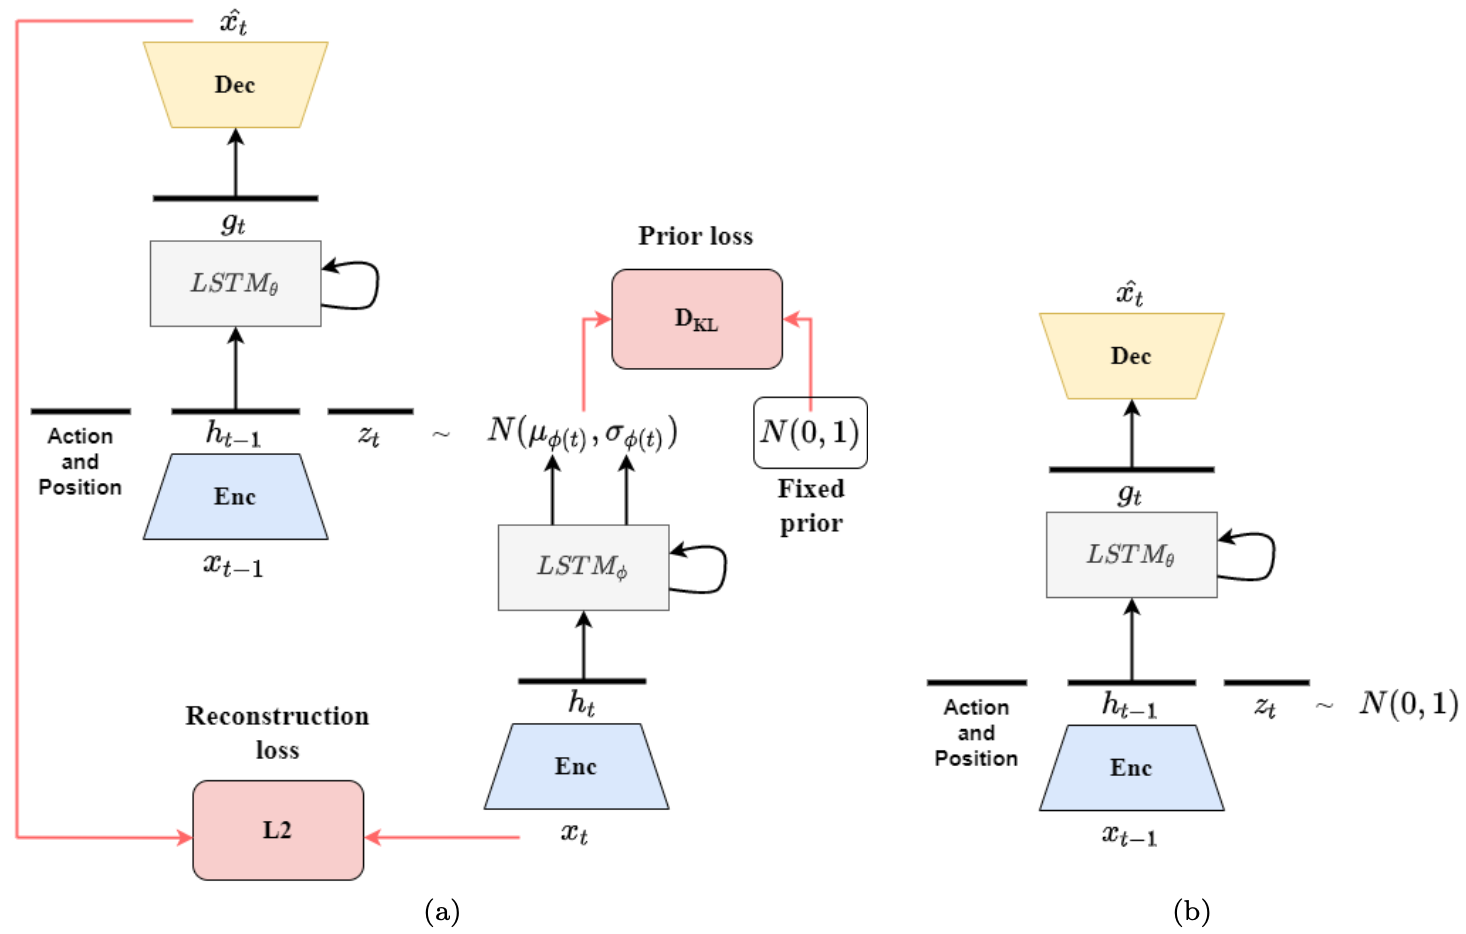
\includegraphics[scale=0.5]{img/architecture.png}
		\caption{Illustration of overall architecture.\\Sub-figure (a) is training procedure, and sub-figure (b) is generation procedure.}
		\label{architecture}
	\end{figure}

\section{Derivation of CVAE}\label{sec-derivation-cvae}
\indent
	Equation \ref{eq-derivation-cvae} is derivation of CVAE objective function.

\begin{equation}\label{eq-derivation-cvae}
	\begin{aligned}
		\mathcal{L} & = \sum_z q_\phi(z)\log\frac{p_\theta(x, z)}{q_\phi(z)} \\
		& = \mathbb{E}_{q_\phi(z)}\log\frac{p_\theta(x, z)}{q_\phi(z)} \\
		& = \mathbb{E}_{q_\phi(z)}\log\frac{p_\theta(x | z)p_\theta(z)}{q_\phi(z)} \\
		& = \mathbb{E}_{q_\phi(z)}\log p_\theta(x | z) + \mathbb{E}_{q_\phi(z)}\log\frac{p_\theta(z)}{q_\phi(z)} \\
		& = \mathbb{E}_{q_\phi(z)}\log p_\theta(x | z) + \text{KL}[q_\phi(z) || p_\theta(z)]
	\end{aligned}
\end{equation}
